
In Citadel, each party involved in the protocol keeps static keys, as we detail now. Let $G, G'\gets\mathbb{J}$ be two generators for the subgroup $\mathbb{J}$ of order $t$ of the Jubjub elliptic curve. The keys of each party are the following.

\begin{itemize}%[label=$\bullet$]
	\item \textit{Secret key:} $\sk = (a,b)$, where $a,b\gets \F_t$.
	\item \textit{Public key:} $\pk = (A,B)$, where $A = a G$ and $B = b G$.
\end{itemize}

The workflow of the Citadel protocol is depicted in Figure \ref{fig:protocol}, and described with full details as follows.

\begin{figure}[h]
	\centering
		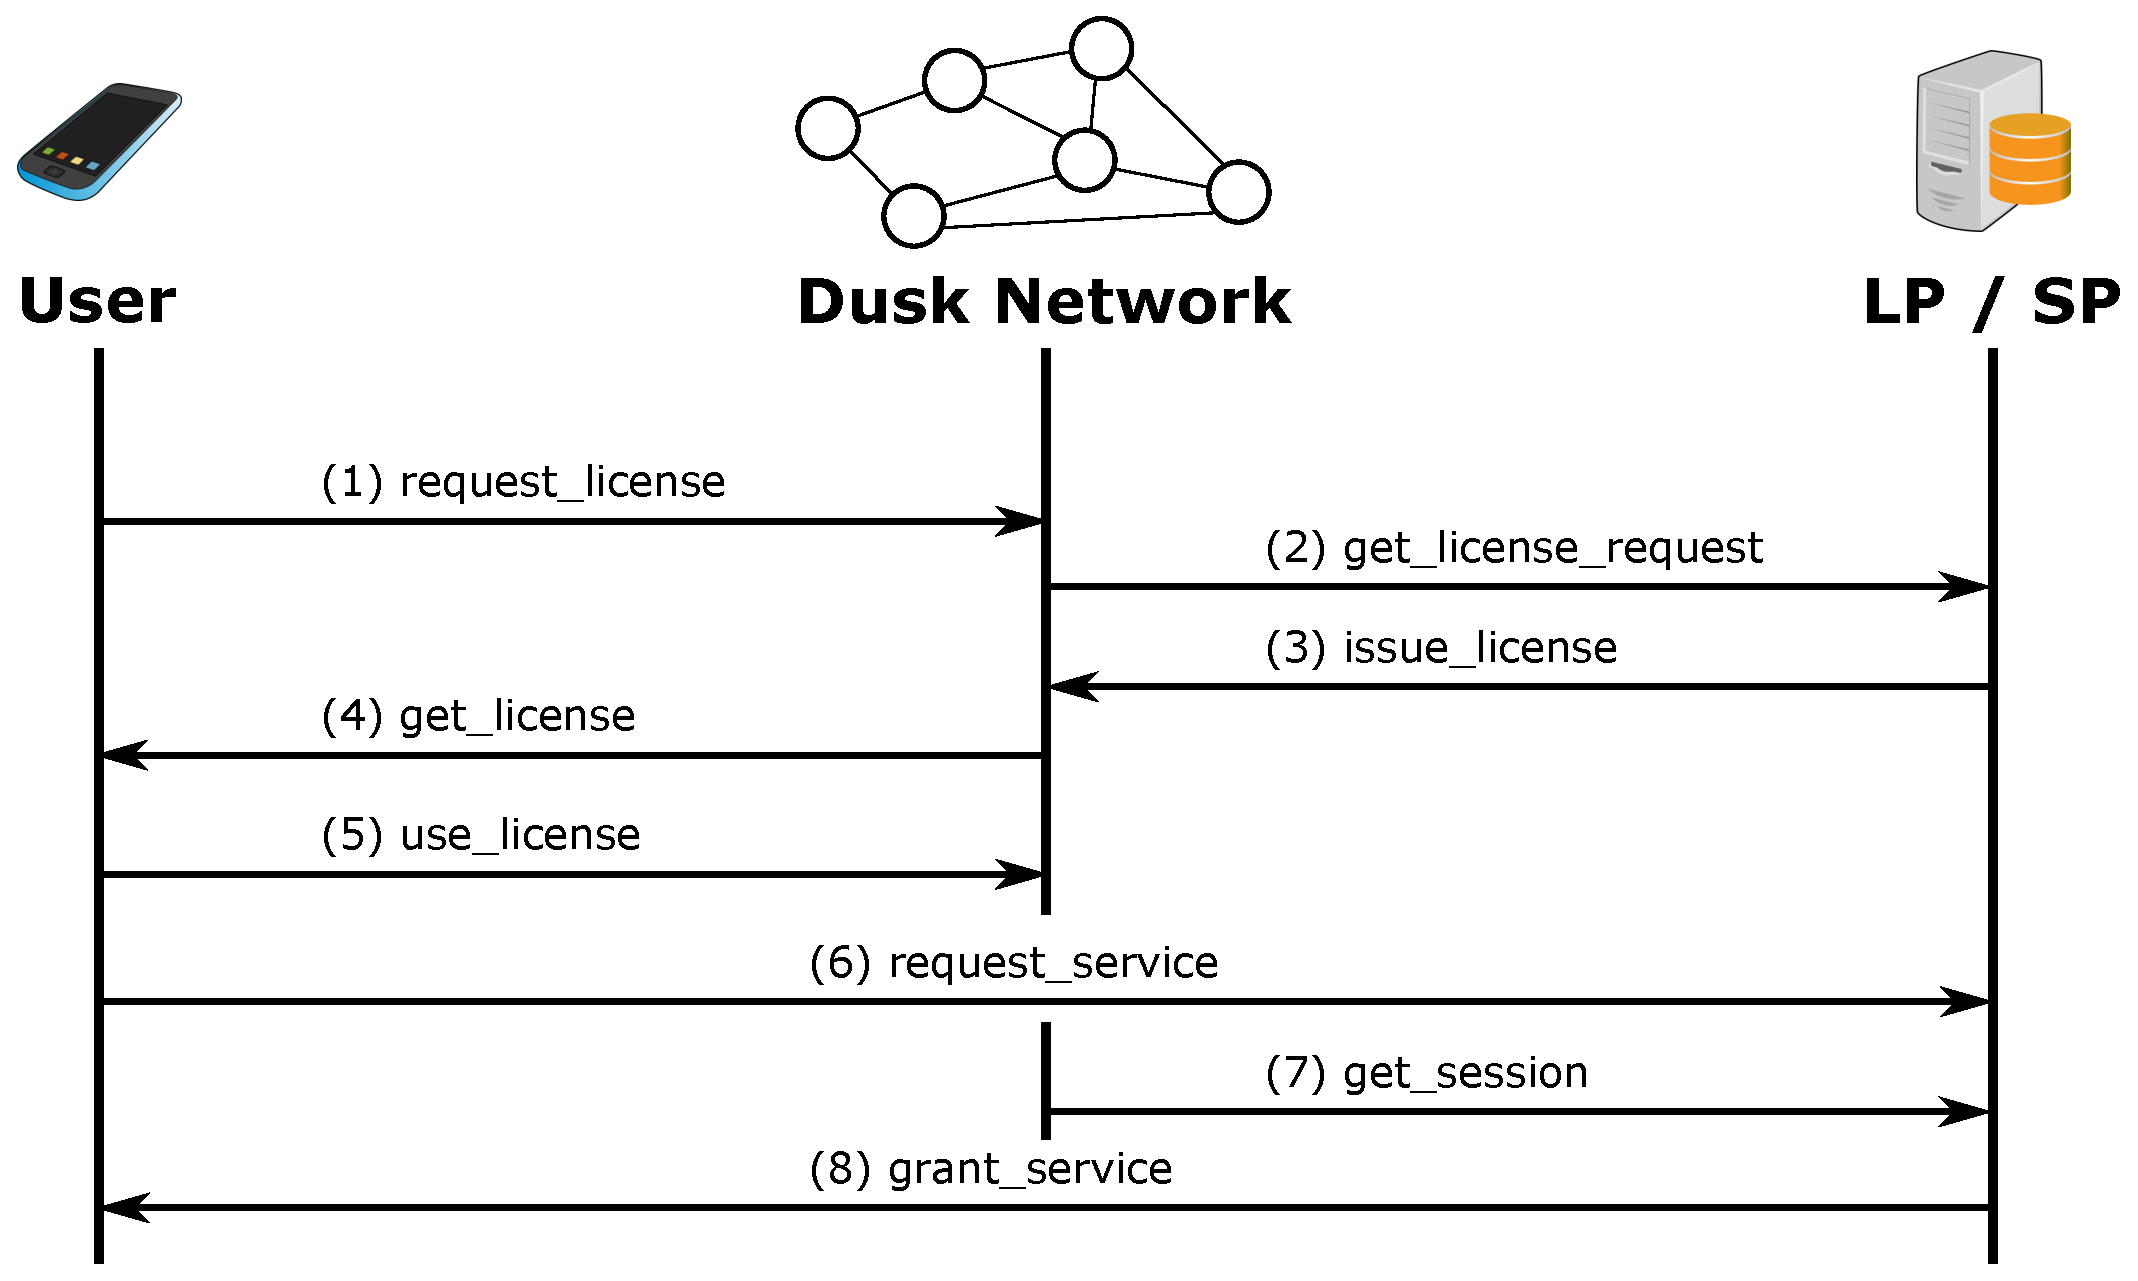
\includegraphics[width=390pt,draft=false]{images/protocol.eps}
	\caption{Overview of the protocol messages exchanged between the user, the Dusk Network, and the SP.}
	\label{fig:protocol}
\end{figure}

\begin{enumerate}
	\item (\textbf{user}) $\mathsf{request\_license}$ : compute a license stealth address $(\lpk, R_{\lic})$ belonging to the user, using the user's own public key, as follows.

	\begin{enumerate}
		\item Sample $r$ uniformly at random from $\F_t$.
		\item Compute a symmetric Diffie--Hellman key $\ksym = rA_{\user}$.
		\item Compute a one-time public key $\lpk = \hb(\ksym)G + B_{\user}$.
		\item Compute $R_{\lic} = rG$.
	\end{enumerate}

	Compute also an additional key $\klic = \hp(\lsk)G$, by computing first the license secret key $\lsk = \hb(\ksym) + b_{\user}$. Then, compute the request stealth address $(\rpk, R_{\req})$ using the LP's public key, as follows.

	\begin{enumerate}
		\item Sample $r$ uniformly at random from $\F_t$.
		\item Compute a symmetric Diffie--Hellman key $\kreq = rA_{\LP}$.
		\item Compute a one-time public key $\rpk = \hb(\kreq)G + B_{\LP}$.
		\item Compute $R_{\req} = rG$.
	\end{enumerate}

	And finally send the following request to the network:

		$$\req = ((\rpk, R_{\req}), \enc, \nonce),$$

	where 

		$$\enc = \Enc_{\kreq} ((\lpk, R_{\lic})||\klic; \nonce).$$


	\item (\textbf{LP}) $\mathsf{get\_license\_request}$ : continuously check the network for incoming license requests, by checking if $\rpk \stackrel{?}{=} \hb(\tkreq) G + B_{\LP}$, where $\tkreq = a_{\LP}R_{\req}$.

	\item (\textbf{LP}) $\mathsf{issue\_license}$ : upon receiving a request from a user, define a set of attributes $\attr$ representing the license, and compute a digital signature as follows:

		$$\lsig = \sign_{\sk_{\SP}}(\lpk, \attr).$$

	Then, send the following license to the network:

		$$\lic = ((\lpk, R_{\lic}), \enc, \nonce, \pos),$$

	where 

		$$\enc = \Enc_{\klic} (\lsig || \attr; \nonce).$$

	\item (\textbf{user}) $\mathsf{get\_license}$ : receive the license by scanning the incoming transactions, and checking if $\lpk \stackrel{?}{=} \hb(\tklic) G + B_{\user}$, where $\tklic = \hb(\lsk)G$.

	\item (\textbf{user}) $\mathsf{use\_license}$ : when using the license, open a session with a specific SP by executing a call to the license contract. The following steps are performed:

	\begin{itemize}
		\item The user issues a transaction that calls the license contract, which includes a ZKP that is computed out of the gadget depicted in Figure \ref{fig:circuit_prove_nft}. Notice that here, the user signs $\mathsf{session\_hash}$ using $\lsk$. Likewise, the user here will need to compute $\lpk' = \lsk G'$.
		\item The network validators will execute the smart contract, which verifies the proof. Upon success, the following session will be added to a shared list of sessions:

			$$\Session = \{\mathsf{session\_hash}, \sessionid, \com_0^{hash}, \com_1, \com_2\},$$

		where $\mathsf{session\_hash} = \hp(\pk_{\SP} || r_\mathsf{session})$, and $r_\mathsf{session}$ is sampled uniformly at random from $\F_t$.


	\end{itemize}

	\item (\textbf{user}) $\mathsf{request\_service}$ : request the service to the SP, establishing communication using a secure channel, and providing the session cookie that follows.

		$$\SessionCookie = \{\pk_{\mathsf{SP}}, r_\mathsf{session}, \sessionid, \pk_{\LP}, \attr, c, \mathsf{s_0}, \mathsf{s_1}, \mathsf{s_2}\}$$

	\item (\textbf{SSP}) $\mathsf{get\_session}$ : receive a $\Session$ from the list of sessions, where $\Session.\sessionid = \SessionCookie.\sessionid$.

	\item (\textbf{SSP}) $\mathsf{grant\_service}$ : grant or deny the service upon verification of the following steps:

	\begin{itemize}
		\item Check whether the values $(\attr, \pk_{\LP}, c)$ included in the $\SessionCookie$ are correct.
		\item Check whether the opening $(\pk_{\SP}, r_\mathsf{session})$ included in the $\SessionCookie$ matches the $\mathsf{session\_hash}$ found in the $\Session$.
		\item Check whether the openings $((\pk_{\LP}, \mathsf{s_0}), (\attr, \mathsf{s_1}), (c, \mathsf{s_2}))$ included in the $\SessionCookie$ match the commitments ($\com_0^{hash}, \com_1, \com_2$) found in the $\Session$.
	\end{itemize}

\end{enumerate}

\begin{figure}[h]
	\centering
	\setlength{\fboxsep}{5pt}%
	\setlength{\fboxrule}{0.3pt}%
	\fbox{
		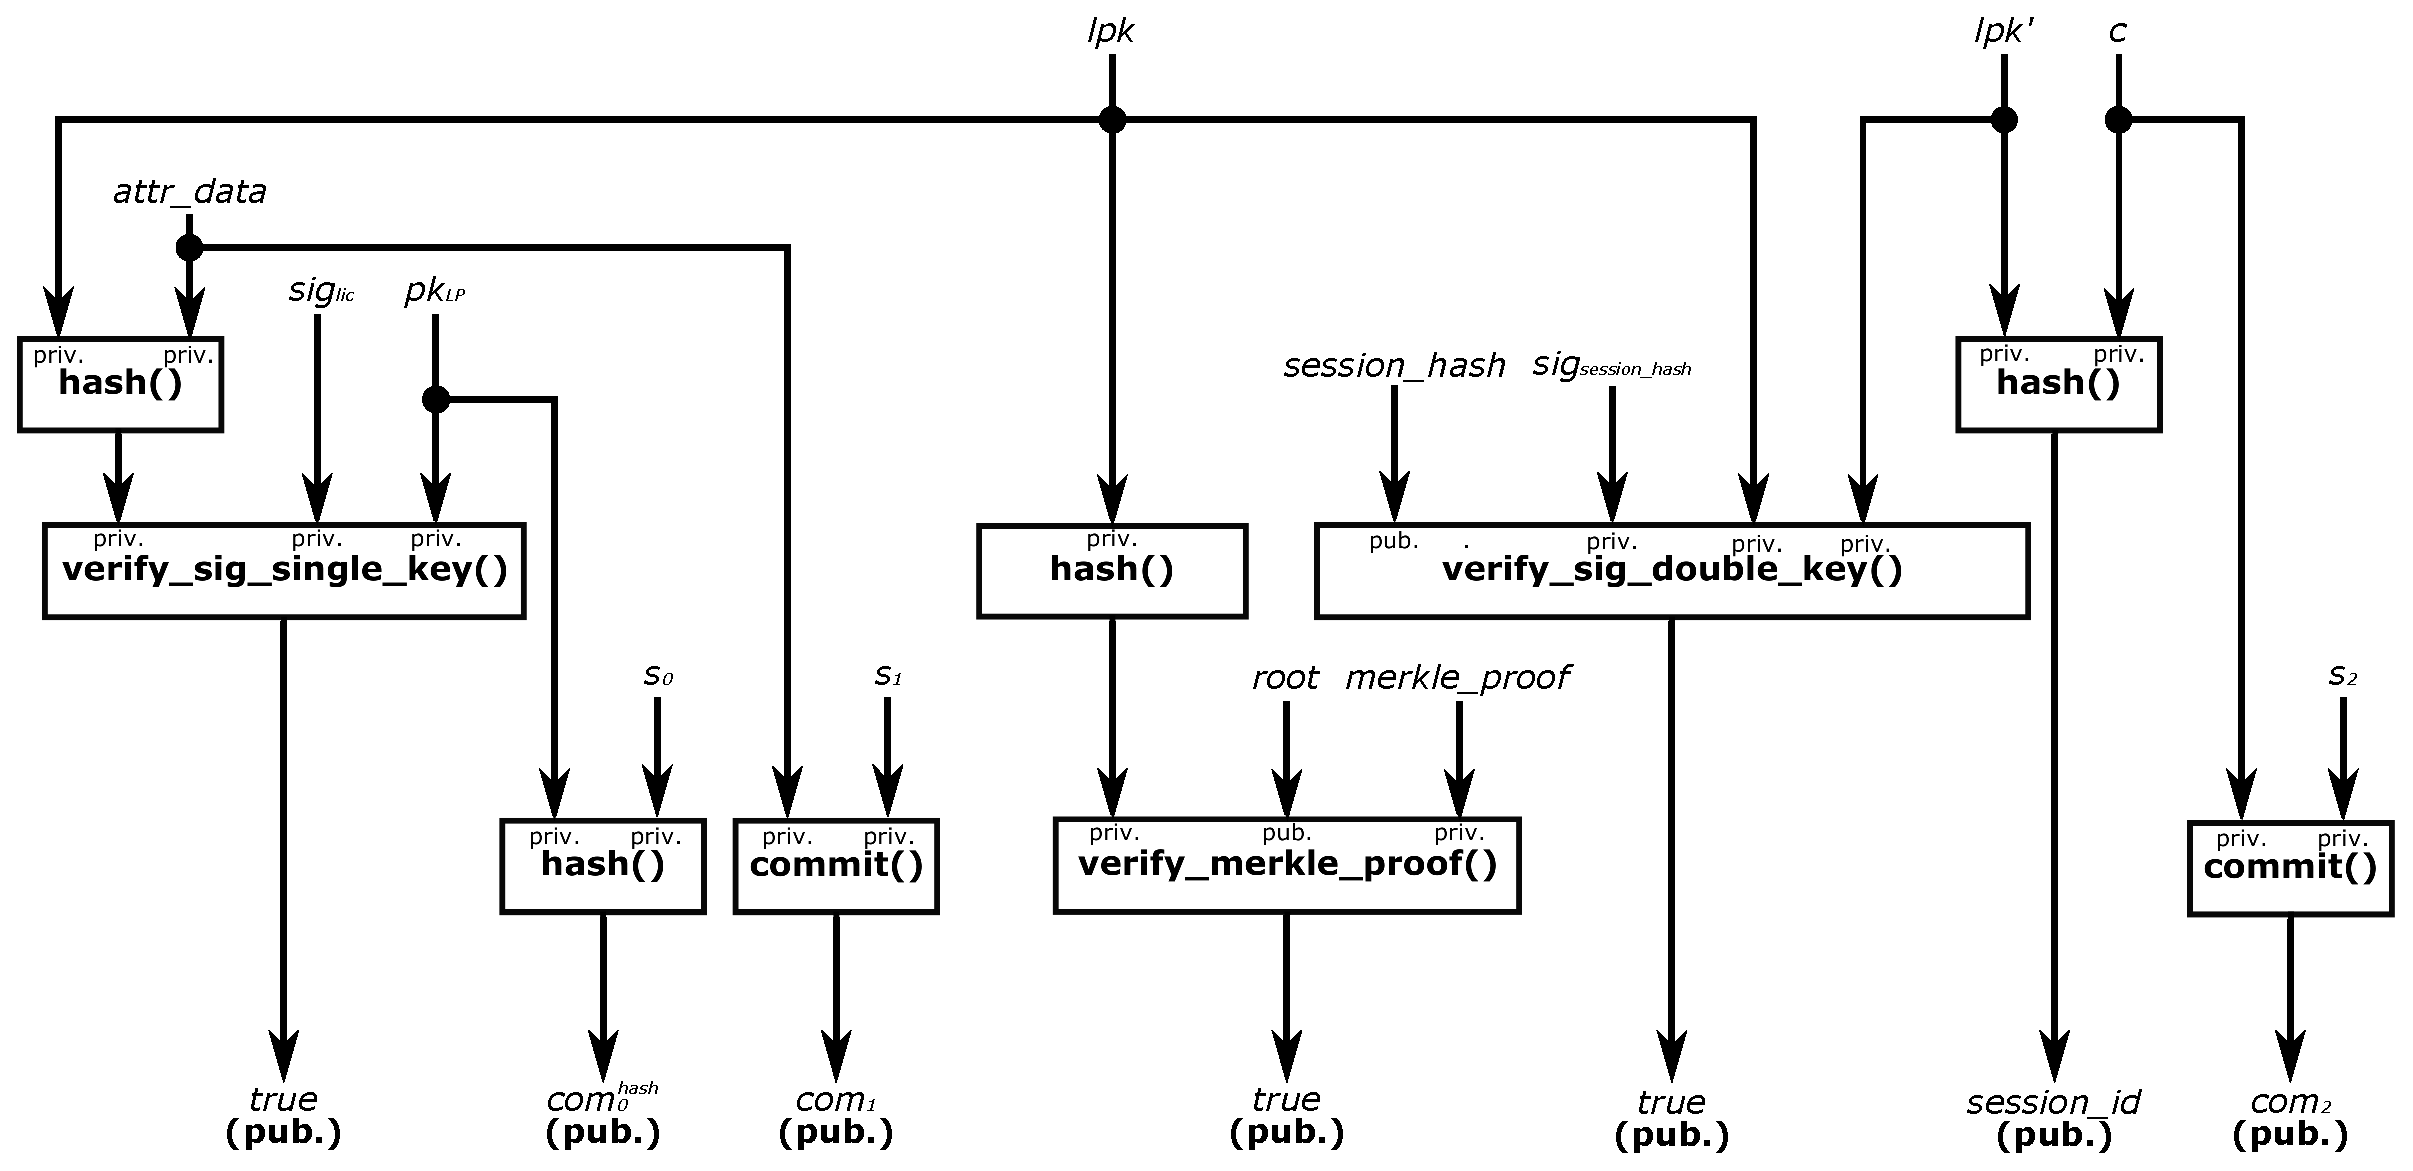
\includegraphics[width=460pt,draft=false]{images/circuit_prove_nft.eps}}
	\caption{Arithmetic circuit for proving a license's ownership.}
	\label{fig:circuit_prove_nft}
\end{figure}

Furthermore, the SP might want to prevent the user from using the license more than once (e.g. this is a single-use license, like entering a concert). This is done through the computation of $\sessionid$. The deployment of this part of the circuit has two different possibilities:
\begin{itemize}
	\item If we set $c = 0$ (or directly remove this input from the circuit), the license can be used only once.
	\item If the SP requests the user to set a custom value for $c$ (e.g. the date of an event), the license can be reused only under certain conditions.
\end{itemize}
